\documentclass[twoside]{book}

% Packages required by doxygen
\usepackage{fixltx2e}
\usepackage{calc}
\usepackage{doxygen}
\usepackage{graphicx}
\usepackage[utf8]{inputenc}
\usepackage{makeidx}
\usepackage{multicol}
\usepackage{multirow}
\PassOptionsToPackage{warn}{textcomp}
\usepackage{textcomp}
\usepackage[nointegrals]{wasysym}
\usepackage[table]{xcolor}

% Font selection
\usepackage[T1]{fontenc}
\usepackage{mathptmx}
\usepackage[scaled=.90]{helvet}
\usepackage{courier}
\usepackage{amssymb}
\usepackage{sectsty}
\renewcommand{\familydefault}{\sfdefault}
\allsectionsfont{%
  \fontseries{bc}\selectfont%
  \color{darkgray}%
}
\renewcommand{\DoxyLabelFont}{%
  \fontseries{bc}\selectfont%
  \color{darkgray}%
}
\newcommand{\+}{\discretionary{\mbox{\scriptsize$\hookleftarrow$}}{}{}}

% Page & text layout
\usepackage{geometry}
\geometry{%
  a4paper,%
  top=2.5cm,%
  bottom=2.5cm,%
  left=2.5cm,%
  right=2.5cm%
}
\tolerance=750
\hfuzz=15pt
\hbadness=750
\setlength{\emergencystretch}{15pt}
\setlength{\parindent}{0cm}
\setlength{\parskip}{0.2cm}
\makeatletter
\renewcommand{\paragraph}{%
  \@startsection{paragraph}{4}{0ex}{-1.0ex}{1.0ex}{%
    \normalfont\normalsize\bfseries\SS@parafont%
  }%
}
\renewcommand{\subparagraph}{%
  \@startsection{subparagraph}{5}{0ex}{-1.0ex}{1.0ex}{%
    \normalfont\normalsize\bfseries\SS@subparafont%
  }%
}
\makeatother

% Headers & footers
\usepackage{fancyhdr}
\pagestyle{fancyplain}
\fancyhead[LE]{\fancyplain{}{\bfseries\thepage}}
\fancyhead[CE]{\fancyplain{}{}}
\fancyhead[RE]{\fancyplain{}{\bfseries\leftmark}}
\fancyhead[LO]{\fancyplain{}{\bfseries\rightmark}}
\fancyhead[CO]{\fancyplain{}{}}
\fancyhead[RO]{\fancyplain{}{\bfseries\thepage}}
\fancyfoot[LE]{\fancyplain{}{}}
\fancyfoot[CE]{\fancyplain{}{}}
\fancyfoot[RE]{\fancyplain{}{\bfseries\scriptsize 2014年12月24日(水) 15時47分33秒作成 -\/ P\+D\+O\+D\+B / 構成\+:  Doxygen }}
\fancyfoot[LO]{\fancyplain{}{\bfseries\scriptsize 2014年12月24日(水) 15時47分33秒作成 -\/ P\+D\+O\+D\+B / 構成\+:  Doxygen }}
\fancyfoot[CO]{\fancyplain{}{}}
\fancyfoot[RO]{\fancyplain{}{}}
\renewcommand{\footrulewidth}{0.4pt}
\renewcommand{\chaptermark}[1]{%
  \markboth{#1}{}%
}
\renewcommand{\sectionmark}[1]{%
  \markright{\thesection\ #1}%
}

% Indices & bibliography
\usepackage{natbib}
\usepackage[titles]{tocloft}
\setcounter{tocdepth}{3}
\setcounter{secnumdepth}{5}
\makeindex

% Hyperlinks (required, but should be loaded last)
\usepackage{ifpdf}
\ifpdf
  \usepackage[pdftex,pagebackref=true]{hyperref}
\else
  \usepackage[ps2pdf,pagebackref=true]{hyperref}
\fi
\hypersetup{%
  colorlinks=true,%
  linkcolor=blue,%
  citecolor=blue,%
  unicode%
}

% Custom commands
\newcommand{\clearemptydoublepage}{%
  \newpage{\pagestyle{empty}\cleardoublepage}%
}


%===== C O N T E N T S =====

\begin{document}

% Titlepage & ToC
\hypersetup{pageanchor=false,
             bookmarks=true,
             bookmarksnumbered=true,
             pdfencoding=unicode
            }
\pagenumbering{roman}
\begin{titlepage}
\vspace*{7cm}
\begin{center}%
{\Large P\+D\+O\+D\+B }\\
\vspace*{1cm}
{\large 構築\+: Doxygen 1.8.8}\\
\vspace*{0.5cm}
{\small 2014年12月24日(水) 15時47分33秒}\\
\end{center}
\end{titlepage}
\clearemptydoublepage
\tableofcontents
\clearemptydoublepage
\pagenumbering{arabic}
\hypersetup{pageanchor=true}

%--- Begin generated contents ---
\chapter{階層索引}
\section{クラス階層}
クラス階層一覧です。大雑把に文字符号順で並べられています。\begin{DoxyCompactList}
\item Exception\begin{DoxyCompactList}
\item \contentsline{section}{Log\+Exception}{\pageref{class_log_exception}}{}
\end{DoxyCompactList}
\item \contentsline{section}{Log}{\pageref{class_log}}{}
\item P\+D\+O\begin{DoxyCompactList}
\item \contentsline{section}{P\+D\+O\+D\+B}{\pageref{class_p_d_o_d_b}}{}
\end{DoxyCompactList}
\end{DoxyCompactList}

\chapter{データ構造索引}
\section{データ構造}
データ構造一覧です。\begin{DoxyCompactList}
\item\contentsline{section}{\hyperlink{class_log}{Log} }{\pageref{class_log}}{}
\item\contentsline{section}{\hyperlink{class_log_exception}{Log\+Exception} }{\pageref{class_log_exception}}{}
\item\contentsline{section}{\hyperlink{class_p_d_o_d_b}{P\+D\+O\+D\+B} }{\pageref{class_p_d_o_d_b}}{}
\end{DoxyCompactList}

\chapter{データ構造詳解}
\hypertarget{class_log}{\section{Log クラス}
\label{class_log}\index{Log@{Log}}
}
\subsection*{公開メンバ関数}
\begin{DoxyCompactItemize}
\item 
\hyperlink{class_log_a67b87fd77dbcba71a2cc1003242b4025}{\+\_\+\+\_\+construct} (\$log\+Nm= 'error.\+log', \$log\+Dir= '.', \$is\+Ym\+Div=T\+R\+U\+E, \$is\+Err\+Disp=T\+R\+U\+E)
\item 
\hyperlink{class_log_aa757d15952223c276bf6355dd20a4c65}{out} ()
\item 
\hyperlink{class_log_a982b6a779ab20914da936c96363ffac3}{get\+Log\+Nm} ()
\item 
\hyperlink{class_log_adf01d6c05e9e80681754d2a9f2bb4cba}{get\+Log\+Full\+Path} ()
\item 
\hyperlink{class_log_ade71d11396892967682c9dc03049a0f3}{get\+Log\+Dir\+Path} ()
\end{DoxyCompactItemize}


\subsection{詳解}
ログクラス

\begin{DoxyVersion}{バージョン}
1.\+1.\+1  U\+T\+F-\/8  2011/02/15  2014/12/24  M\+I\+T 
\end{DoxyVersion}
\begin{DoxyAuthor}{著者}
mamiya\+\_\+shou 
\end{DoxyAuthor}
\begin{DoxyCopyright}{著作権所有}
mamiya\+\_\+shou  P\+H\+P 5.\+0 以上必須 
\end{DoxyCopyright}


\subsection{構築子と解体子}
\hypertarget{class_log_a67b87fd77dbcba71a2cc1003242b4025}{\index{Log@{Log}!\+\_\+\+\_\+construct@{\+\_\+\+\_\+construct}}
\index{\+\_\+\+\_\+construct@{\+\_\+\+\_\+construct}!Log@{Log}}
\subsubsection[{\+\_\+\+\_\+construct}]{\setlength{\rightskip}{0pt plus 5cm}\+\_\+\+\_\+construct (
\begin{DoxyParamCaption}
\item[{}]{\$log\+Nm = {\ttfamily 'error.log'}, }
\item[{}]{\$log\+Dir = {\ttfamily '.'}, }
\item[{}]{\$is\+Ym\+Div = {\ttfamily TRUE}, }
\item[{}]{\$is\+Err\+Disp = {\ttfamily TRUE}}
\end{DoxyParamCaption}
)}}\label{class_log_a67b87fd77dbcba71a2cc1003242b4025}
エラー時にメッセージを表示するかどうか コンストラクタ


\begin{DoxyParams}[1]{引数}
string & {\em \$log\+Nm} & ログファイル名 (def\+:'error.\+log') \\
\hline
string & {\em \$log\+Dir} & ログファイルのディレクトリ (def\+:'.') \\
\hline
boolean & {\em \$is\+Ym\+Div} & ログファイル名に年月を追加してファイル分けるかどうか (def\+:T\+R\+U\+E) \\
\hline
boolean & {\em \$is\+Err\+Disp} & エラー時にメッセージを表示するかどうか (def\+:T\+R\+U\+E) \\
\hline
\end{DoxyParams}


\subsection{関数詳解}
\hypertarget{class_log_ade71d11396892967682c9dc03049a0f3}{\index{Log@{Log}!get\+Log\+Dir\+Path@{get\+Log\+Dir\+Path}}
\index{get\+Log\+Dir\+Path@{get\+Log\+Dir\+Path}!Log@{Log}}
\subsubsection[{get\+Log\+Dir\+Path}]{\setlength{\rightskip}{0pt plus 5cm}get\+Log\+Dir\+Path (
\begin{DoxyParamCaption}
{}
\end{DoxyParamCaption}
)}}\label{class_log_ade71d11396892967682c9dc03049a0f3}
ログディレクトリのパスを返す

\begin{DoxyReturn}{戻り値}
string ログディレクトリのパス 
\end{DoxyReturn}
\hypertarget{class_log_adf01d6c05e9e80681754d2a9f2bb4cba}{\index{Log@{Log}!get\+Log\+Full\+Path@{get\+Log\+Full\+Path}}
\index{get\+Log\+Full\+Path@{get\+Log\+Full\+Path}!Log@{Log}}
\subsubsection[{get\+Log\+Full\+Path}]{\setlength{\rightskip}{0pt plus 5cm}get\+Log\+Full\+Path (
\begin{DoxyParamCaption}
{}
\end{DoxyParamCaption}
)}}\label{class_log_adf01d6c05e9e80681754d2a9f2bb4cba}
ログファイルのフルパスを返す

\begin{DoxyReturn}{戻り値}
string ログファイルのフルパス 
\end{DoxyReturn}
\hypertarget{class_log_a982b6a779ab20914da936c96363ffac3}{\index{Log@{Log}!get\+Log\+Nm@{get\+Log\+Nm}}
\index{get\+Log\+Nm@{get\+Log\+Nm}!Log@{Log}}
\subsubsection[{get\+Log\+Nm}]{\setlength{\rightskip}{0pt plus 5cm}get\+Log\+Nm (
\begin{DoxyParamCaption}
{}
\end{DoxyParamCaption}
)}}\label{class_log_a982b6a779ab20914da936c96363ffac3}
ログファイル名を返す

\begin{DoxyReturn}{戻り値}
string ログファイルのフルパス 
\end{DoxyReturn}
\hypertarget{class_log_aa757d15952223c276bf6355dd20a4c65}{\index{Log@{Log}!out@{out}}
\index{out@{out}!Log@{Log}}
\subsubsection[{out}]{\setlength{\rightskip}{0pt plus 5cm}out (
\begin{DoxyParamCaption}
{}
\end{DoxyParamCaption}
)}}\label{class_log_aa757d15952223c276bf6355dd20a4c65}
ログファイルに書き込む

\begin{DoxyReturn}{戻り値}
boolean 書き込みの成否  引数に指定されたモノをカンマで結合し出力 
\end{DoxyReturn}


このクラス詳解は次のファイルから抽出されました\+:\begin{DoxyCompactItemize}
\item 
P\+D\+O\+D\+B/\+Log/Log.\+php\end{DoxyCompactItemize}

\hypertarget{class_log_exception}{\section{Log\+Exception クラス}
\label{class_log_exception}\index{Log\+Exception@{Log\+Exception}}
}
Log\+Exception の継承関係図\begin{figure}[H]
\begin{center}
\leavevmode
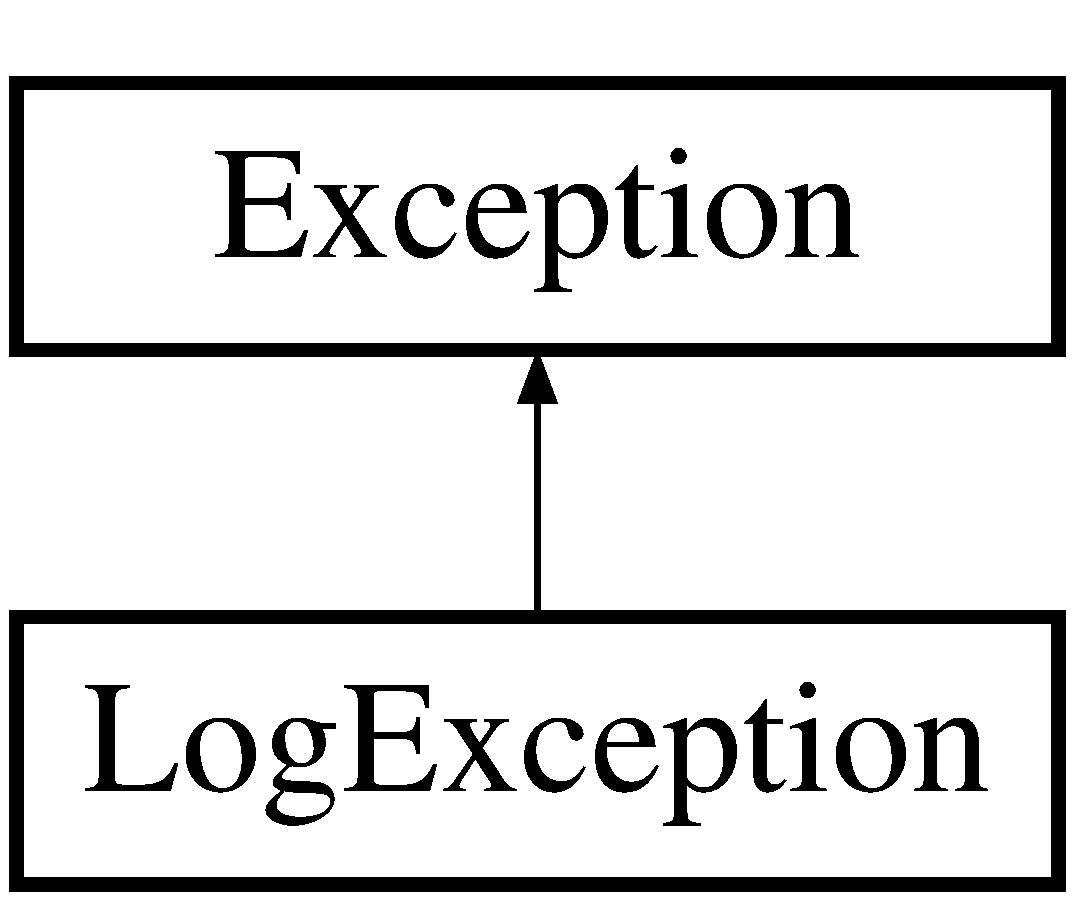
\includegraphics[height=2.000000cm]{class_log_exception}
\end{center}
\end{figure}


\subsection{詳解}
Log\+Exceptionクラス

Exceptionクラスを継承 

このクラス詳解は次のファイルから抽出されました\+:\begin{DoxyCompactItemize}
\item 
P\+D\+O\+D\+B/\+Log/Log.\+php\end{DoxyCompactItemize}

\hypertarget{class_p_d_o_d_b}{\section{P\+D\+O\+D\+B クラス}
\label{class_p_d_o_d_b}\index{P\+D\+O\+D\+B@{P\+D\+O\+D\+B}}
}
P\+D\+O\+D\+B の継承関係図\begin{figure}[H]
\begin{center}
\leavevmode
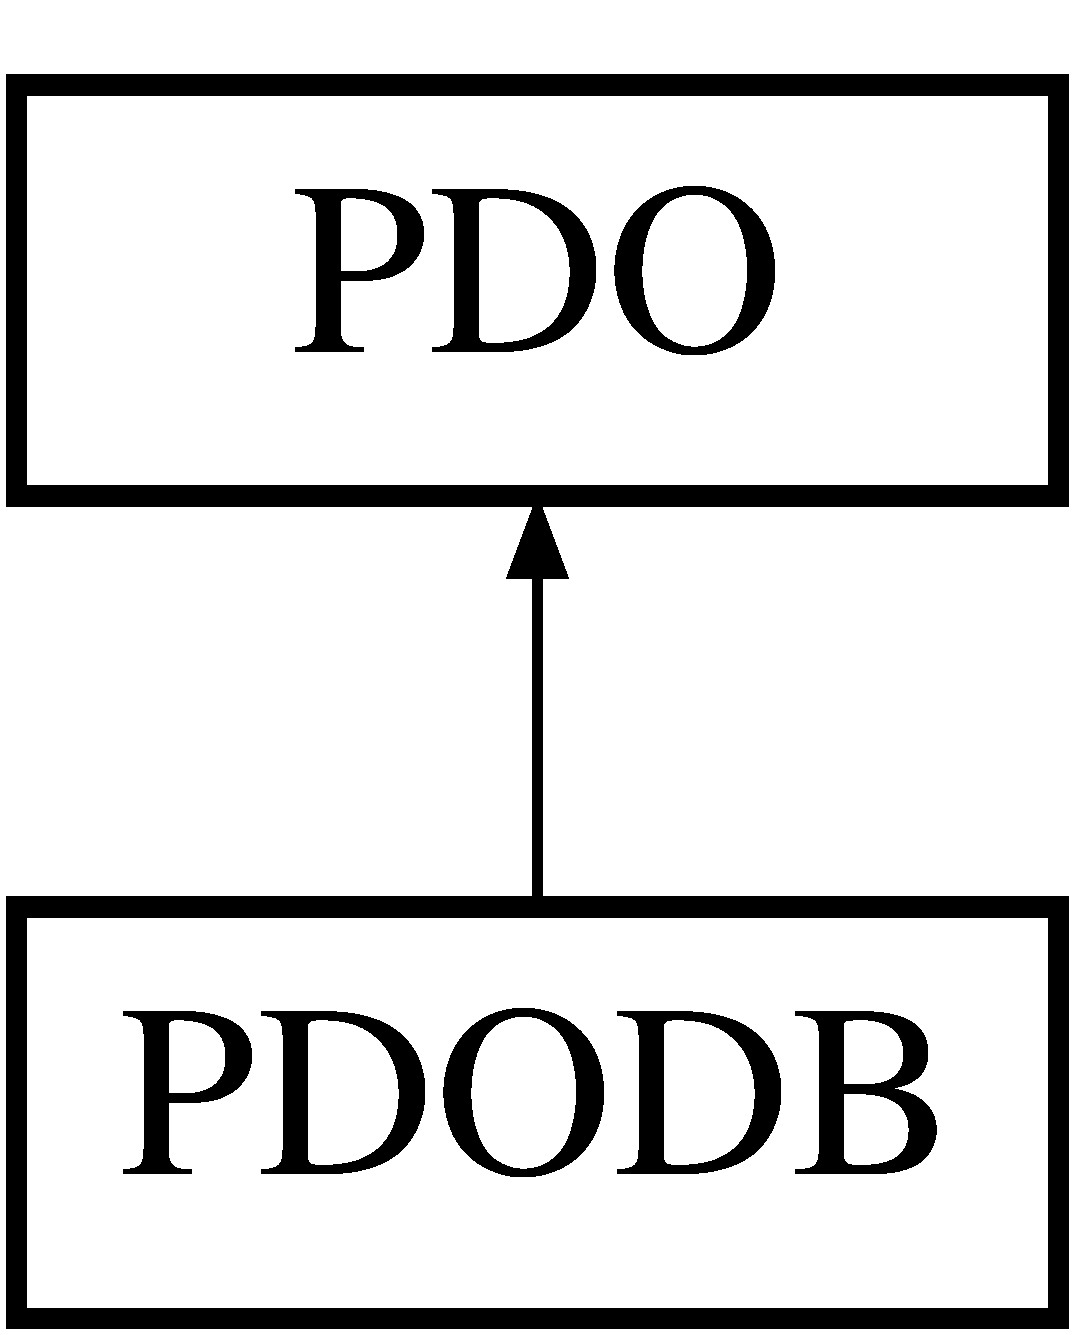
\includegraphics[height=2.000000cm]{class_p_d_o_d_b}
\end{center}
\end{figure}
\subsection*{公開メンバ関数}
\begin{DoxyCompactItemize}
\item 
\hyperlink{class_p_d_o_d_b_ab83ddb38397a6269ad9889763849375b}{\+\_\+\+\_\+construct} (\$db\+Nm, \$is\+Err\+Disp=T\+R\+U\+E, \$is\+Connect=T\+R\+U\+E)
\item 
\hyperlink{class_p_d_o_d_b_a659097eced6535d165a7a53e58965a32}{connect} (\$db\+Nm, \$is\+Err\+Disp=T\+R\+U\+E)
\item 
\hyperlink{class_p_d_o_d_b_a77a6eabc05971e2d9e2d27c834fa7fd7}{select} (\$fld=N\+U\+L\+L, \$table=N\+U\+L\+L, \$where=N\+U\+L\+L, \$ary\+Bind=N\+U\+L\+L, \$option=N\+U\+L\+L)
\item 
\hyperlink{class_p_d_o_d_b_a9afeeb57a89e5635a431de8e5b542064}{select\+All} (\$fld=N\+U\+L\+L, \$table=N\+U\+L\+L, \$where=N\+U\+L\+L, \$ary\+Bind=N\+U\+L\+L, \$option=N\+U\+L\+L)
\item 
\hyperlink{class_p_d_o_d_b_ac4ebdc9ea23cdaa05830bc1c24a49935}{insert} (\$ary\+Fld=N\+U\+L\+L, \$table=N\+U\+L\+L, \$ary\+Bind=N\+U\+L\+L)
\item 
\hyperlink{class_p_d_o_d_b_a179ba8695e7f6322edbdf57f6f5f6877}{update} (\$ary\+Fld=N\+U\+L\+L, \$table=N\+U\+L\+L, \$where=N\+U\+L\+L, \$ary\+Bind=N\+U\+L\+L)
\item 
\hyperlink{class_p_d_o_d_b_a86b899c21ecfb0135557d0222ac5dfa7}{delete} (\$table=N\+U\+L\+L, \$where=N\+U\+L\+L, \$ary\+Bind=N\+U\+L\+L)
\item 
\hyperlink{class_p_d_o_d_b_a0f84f6939001f98d3c4bffc48def826e}{wild\+Card\+Quote} (\$str)
\item 
\hyperlink{class_p_d_o_d_b_aa6d5dabec08e65836e680cc996882850}{prepara\+Mode} ()
\item 
\hyperlink{class_p_d_o_d_b_a67e8cb12dd05cee2a73454f8fa79efdc}{get\+S\+Q\+L} ()
\item 
\hyperlink{class_p_d_o_d_b_a9eb561b3798add7d463b192f8057fde7}{write\+Exception} (\$e, \$ary\+Debug=N\+U\+L\+L)
\end{DoxyCompactItemize}
\subsection*{フィールド}
\begin{DoxyCompactItemize}
\item 
\hypertarget{class_p_d_o_d_b_a047170d6020a882807665812a27e2525}{{\bfseries \$sql}}\label{class_p_d_o_d_b_a047170d6020a882807665812a27e2525}

\item 
\hypertarget{class_p_d_o_d_b_a139dfb0d4211dd1706570778a5a9d692}{{\bfseries \$ary\+Bind}}\label{class_p_d_o_d_b_a139dfb0d4211dd1706570778a5a9d692}

\item 
\hypertarget{class_p_d_o_d_b_aa9c41fca31d8871ad2fe81c45a5963a5}{{\bfseries \$pre\+Sql}}\label{class_p_d_o_d_b_aa9c41fca31d8871ad2fe81c45a5963a5}

\item 
\hypertarget{class_p_d_o_d_b_abb05cef0bb5ac558ae5211a3c419e2fc}{{\bfseries \$ary\+Pre\+Bind}}\label{class_p_d_o_d_b_abb05cef0bb5ac558ae5211a3c419e2fc}

\item 
\hypertarget{class_p_d_o_d_b_a6b7e8055dba3b29240adc7b8b7f22bba}{{\bfseries \$is\+Err\+Disp}}\label{class_p_d_o_d_b_a6b7e8055dba3b29240adc7b8b7f22bba}

\end{DoxyCompactItemize}


\subsection{詳解}
P\+D\+O\+D\+Bクラス

\begin{DoxyVersion}{バージョン}
1.\+1.\+0  U\+T\+F-\/8  2010/10/03  2014/12/24 
\end{DoxyVersion}
\begin{DoxyAuthor}{著者}
mamiya\+\_\+shou  mamiya\+\_\+shou  M\+I\+T License 
\begin{DoxyItemize}
\item P\+D\+Oクラスを継承。
\item プレースホルダ機能を使う場合は、外部指定用\+S\+Q\+Lとバインド配列を使うこと。  P\+H\+P 5.\+1.\+0 以上必須 以下のファイルは必須 P\+D\+O\+D\+B.\+ini.\+php P\+D\+O\+D\+Bクラスの設定ファイル Log.\+php ログクラス 
\end{DoxyItemize}
\end{DoxyAuthor}


\subsection{構築子と解体子}
\hypertarget{class_p_d_o_d_b_ab83ddb38397a6269ad9889763849375b}{\index{P\+D\+O\+D\+B@{P\+D\+O\+D\+B}!\+\_\+\+\_\+construct@{\+\_\+\+\_\+construct}}
\index{\+\_\+\+\_\+construct@{\+\_\+\+\_\+construct}!P\+D\+O\+D\+B@{P\+D\+O\+D\+B}}
\subsubsection[{\+\_\+\+\_\+construct}]{\setlength{\rightskip}{0pt plus 5cm}\+\_\+\+\_\+construct (
\begin{DoxyParamCaption}
\item[{}]{\$db\+Nm, }
\item[{}]{\$is\+Err\+Disp = {\ttfamily TRUE}, }
\item[{}]{\$is\+Connect = {\ttfamily TRUE}}
\end{DoxyParamCaption}
)}}\label{class_p_d_o_d_b_ab83ddb38397a6269ad9889763849375b}
コンストラクタ


\begin{DoxyParams}[1]{引数}
string & {\em \$db\+Nm} & P\+D\+O\+D\+B.\+ini.\+php で定義された \$ary\+Info\+D\+B のキー値 \\
\hline
boolean & {\em \$is\+Err\+Disp} & エラー表示設定 (def\+:T\+R\+U\+E) \\
\hline
boolean & {\em \$is\+Connect} & D\+Bに接続するか否か (def\+:T\+R\+U\+E) \\
\hline
\end{DoxyParams}


\subsection{関数詳解}
\hypertarget{class_p_d_o_d_b_a659097eced6535d165a7a53e58965a32}{\index{P\+D\+O\+D\+B@{P\+D\+O\+D\+B}!connect@{connect}}
\index{connect@{connect}!P\+D\+O\+D\+B@{P\+D\+O\+D\+B}}
\subsubsection[{connect}]{\setlength{\rightskip}{0pt plus 5cm}connect (
\begin{DoxyParamCaption}
\item[{}]{\$db\+Nm, }
\item[{}]{\$is\+Err\+Disp = {\ttfamily TRUE}}
\end{DoxyParamCaption}
)}}\label{class_p_d_o_d_b_a659097eced6535d165a7a53e58965a32}
D\+Bに接続する


\begin{DoxyParams}[1]{引数}
string & {\em \$db\+Nm} & P\+D\+O\+D\+B.\+ini.\+php で定義された \$ary\+Info\+D\+B のキー値 \\
\hline
 & {\em boolean} & エラー表示フラグ \\
\hline
\end{DoxyParams}
\begin{DoxyReturn}{戻り値}
void  D\+Bの接続先を変える際はこのメソッドを使用する 
\end{DoxyReturn}
\hypertarget{class_p_d_o_d_b_a86b899c21ecfb0135557d0222ac5dfa7}{\index{P\+D\+O\+D\+B@{P\+D\+O\+D\+B}!delete@{delete}}
\index{delete@{delete}!P\+D\+O\+D\+B@{P\+D\+O\+D\+B}}
\subsubsection[{delete}]{\setlength{\rightskip}{0pt plus 5cm}delete (
\begin{DoxyParamCaption}
\item[{}]{\$table = {\ttfamily NULL}, }
\item[{}]{\$where = {\ttfamily NULL}, }
\item[{}]{\$ary\+Bind = {\ttfamily NULL}}
\end{DoxyParamCaption}
)}}\label{class_p_d_o_d_b_a86b899c21ecfb0135557d0222ac5dfa7}
データを削除する


\begin{DoxyParams}{引数}
{\em \$table} & テーブル \\
\hline
{\em \$where} & W\+H\+E\+R\+E句 \\
\hline
{\em \$ary\+Bind} & バインド配列 \\
\hline
\end{DoxyParams}
\begin{DoxyReturn}{戻り値}
削除した行数 / 例外発生(失敗) 
\end{DoxyReturn}
\hypertarget{class_p_d_o_d_b_a67e8cb12dd05cee2a73454f8fa79efdc}{\index{P\+D\+O\+D\+B@{P\+D\+O\+D\+B}!get\+S\+Q\+L@{get\+S\+Q\+L}}
\index{get\+S\+Q\+L@{get\+S\+Q\+L}!P\+D\+O\+D\+B@{P\+D\+O\+D\+B}}
\subsubsection[{get\+S\+Q\+L}]{\setlength{\rightskip}{0pt plus 5cm}get\+S\+Q\+L (
\begin{DoxyParamCaption}
{}
\end{DoxyParamCaption}
)}}\label{class_p_d_o_d_b_a67e8cb12dd05cee2a73454f8fa79efdc}
直前に実行した\+S\+Q\+L文を取得する

\begin{DoxyReturn}{戻り値}
array 直前に実行した\+S\+Q\+L情報配列 
\end{DoxyReturn}
\hypertarget{class_p_d_o_d_b_ac4ebdc9ea23cdaa05830bc1c24a49935}{\index{P\+D\+O\+D\+B@{P\+D\+O\+D\+B}!insert@{insert}}
\index{insert@{insert}!P\+D\+O\+D\+B@{P\+D\+O\+D\+B}}
\subsubsection[{insert}]{\setlength{\rightskip}{0pt plus 5cm}insert (
\begin{DoxyParamCaption}
\item[{}]{\$ary\+Fld = {\ttfamily NULL}, }
\item[{}]{\$table = {\ttfamily NULL}, }
\item[{}]{\$ary\+Bind = {\ttfamily NULL}}
\end{DoxyParamCaption}
)}}\label{class_p_d_o_d_b_ac4ebdc9ea23cdaa05830bc1c24a49935}
データを追加する


\begin{DoxyParams}{引数}
{\em \$ary\+Fld} & フィールド配列 \\
\hline
{\em \$table} & テーブル \\
\hline
{\em \$ary\+Bind} & バインド配列 \\
\hline
\end{DoxyParams}
\begin{DoxyReturn}{戻り値}
T\+R\+U\+E(\+O\+K) / 例外発生(\+N\+G) 
\end{DoxyReturn}
\hypertarget{class_p_d_o_d_b_aa6d5dabec08e65836e680cc996882850}{\index{P\+D\+O\+D\+B@{P\+D\+O\+D\+B}!prepara\+Mode@{prepara\+Mode}}
\index{prepara\+Mode@{prepara\+Mode}!P\+D\+O\+D\+B@{P\+D\+O\+D\+B}}
\subsubsection[{prepara\+Mode}]{\setlength{\rightskip}{0pt plus 5cm}prepara\+Mode (
\begin{DoxyParamCaption}
{}
\end{DoxyParamCaption}
)}}\label{class_p_d_o_d_b_aa6d5dabec08e65836e680cc996882850}
プリペアドステートメントモードを設定する


\begin{DoxyParams}[1]{引数}
boolean & {\em \$mode} & プリペアドステートメントモード  プリペアドステートメントモードは\+S\+Q\+L実行後、自動的に\+F\+A\+L\+S\+Eに設定される \\
\hline
\end{DoxyParams}
\hypertarget{class_p_d_o_d_b_a77a6eabc05971e2d9e2d27c834fa7fd7}{\index{P\+D\+O\+D\+B@{P\+D\+O\+D\+B}!select@{select}}
\index{select@{select}!P\+D\+O\+D\+B@{P\+D\+O\+D\+B}}
\subsubsection[{select}]{\setlength{\rightskip}{0pt plus 5cm}select (
\begin{DoxyParamCaption}
\item[{}]{\$fld = {\ttfamily NULL}, }
\item[{}]{\$table = {\ttfamily NULL}, }
\item[{}]{\$where = {\ttfamily NULL}, }
\item[{}]{\$ary\+Bind = {\ttfamily NULL}, }
\item[{}]{\$option = {\ttfamily NULL}}
\end{DoxyParamCaption}
)}}\label{class_p_d_o_d_b_a77a6eabc05971e2d9e2d27c834fa7fd7}
データを単一取得する


\begin{DoxyParams}[1]{引数}
string & {\em \$fld} & フィールド \\
\hline
string & {\em \$table} & テーブル \\
\hline
string & {\em \$where} & W\+H\+E\+R\+E句 \\
\hline
array & {\em \$ary\+Bind} & バインドする配列 \\
\hline
string & {\em \$option} & オプション(\+O\+R\+D\+E\+R B\+Y, L\+I\+M\+I\+T, O\+F\+F\+S\+E\+T) \\
\hline
\end{DoxyParams}
\begin{DoxyReturn}{戻り値}
object 結果オブジェクト / boolean F\+A\+L\+S\+E(取得する行がない場合) 
\end{DoxyReturn}
\hypertarget{class_p_d_o_d_b_a9afeeb57a89e5635a431de8e5b542064}{\index{P\+D\+O\+D\+B@{P\+D\+O\+D\+B}!select\+All@{select\+All}}
\index{select\+All@{select\+All}!P\+D\+O\+D\+B@{P\+D\+O\+D\+B}}
\subsubsection[{select\+All}]{\setlength{\rightskip}{0pt plus 5cm}select\+All (
\begin{DoxyParamCaption}
\item[{}]{\$fld = {\ttfamily NULL}, }
\item[{}]{\$table = {\ttfamily NULL}, }
\item[{}]{\$where = {\ttfamily NULL}, }
\item[{}]{\$ary\+Bind = {\ttfamily NULL}, }
\item[{}]{\$option = {\ttfamily NULL}}
\end{DoxyParamCaption}
)}}\label{class_p_d_o_d_b_a9afeeb57a89e5635a431de8e5b542064}
データを複数取得する


\begin{DoxyParams}[1]{引数}
string & {\em \$fld} & フィールド \\
\hline
string & {\em \$table} & テーブル \\
\hline
string & {\em \$where} & W\+H\+E\+R\+E句 \\
\hline
array & {\em \$ary\+Bind} & バインドする配列 \\
\hline
string & {\em \$option} & オプション(\+O\+R\+D\+E\+R B\+Y, L\+I\+M\+I\+T, O\+F\+F\+S\+E\+T) \\
\hline
\end{DoxyParams}
\begin{DoxyReturn}{戻り値}
arrary object 結果オブジェクト配列 
\end{DoxyReturn}
\hypertarget{class_p_d_o_d_b_a179ba8695e7f6322edbdf57f6f5f6877}{\index{P\+D\+O\+D\+B@{P\+D\+O\+D\+B}!update@{update}}
\index{update@{update}!P\+D\+O\+D\+B@{P\+D\+O\+D\+B}}
\subsubsection[{update}]{\setlength{\rightskip}{0pt plus 5cm}update (
\begin{DoxyParamCaption}
\item[{}]{\$ary\+Fld = {\ttfamily NULL}, }
\item[{}]{\$table = {\ttfamily NULL}, }
\item[{}]{\$where = {\ttfamily NULL}, }
\item[{}]{\$ary\+Bind = {\ttfamily NULL}}
\end{DoxyParamCaption}
)}}\label{class_p_d_o_d_b_a179ba8695e7f6322edbdf57f6f5f6877}
データを更新する


\begin{DoxyParams}{引数}
{\em \$ary\+Fld} & フィールド配列 \\
\hline
{\em \$table} & テーブル \\
\hline
{\em \$where} & W\+H\+E\+R\+E句 \\
\hline
{\em \$ary\+Bind} & バインド配列 \\
\hline
\end{DoxyParams}
\begin{DoxyReturn}{戻り値}
更新した行数 / 例外発生(失敗) 
\end{DoxyReturn}
\hypertarget{class_p_d_o_d_b_a0f84f6939001f98d3c4bffc48def826e}{\index{P\+D\+O\+D\+B@{P\+D\+O\+D\+B}!wild\+Card\+Quote@{wild\+Card\+Quote}}
\index{wild\+Card\+Quote@{wild\+Card\+Quote}!P\+D\+O\+D\+B@{P\+D\+O\+D\+B}}
\subsubsection[{wild\+Card\+Quote}]{\setlength{\rightskip}{0pt plus 5cm}wild\+Card\+Quote (
\begin{DoxyParamCaption}
\item[{}]{\$str}
\end{DoxyParamCaption}
)}}\label{class_p_d_o_d_b_a0f84f6939001f98d3c4bffc48def826e}
ワイルドカード「\+\_\+」「」をクォートする


\begin{DoxyParams}[1]{引数}
string & {\em \$str} & ワイルドカードが含まれる文字列 \\
\hline
\end{DoxyParams}
\begin{DoxyReturn}{戻り値}
string クォート後の文字列 
\end{DoxyReturn}
\hypertarget{class_p_d_o_d_b_a9eb561b3798add7d463b192f8057fde7}{\index{P\+D\+O\+D\+B@{P\+D\+O\+D\+B}!write\+Exception@{write\+Exception}}
\index{write\+Exception@{write\+Exception}!P\+D\+O\+D\+B@{P\+D\+O\+D\+B}}
\subsubsection[{write\+Exception}]{\setlength{\rightskip}{0pt plus 5cm}write\+Exception (
\begin{DoxyParamCaption}
\item[{}]{\$e, }
\item[{}]{\$ary\+Debug = {\ttfamily NULL}}
\end{DoxyParamCaption}
)}}\label{class_p_d_o_d_b_a9eb561b3798add7d463b192f8057fde7}
例外内容を出力する


\begin{DoxyParams}[1]{引数}
object & {\em \$e} & 例外オブジェクト \\
\hline
array & {\em \$ary\+Debug} & 呼び出し元で\+Callしたdebug\+\_\+backtrace()の戻り値 \\
\hline
\end{DoxyParams}
\begin{DoxyReturn}{戻り値}
void 
\end{DoxyReturn}

\begin{DoxyExceptions}{例外}
{\em P\+D\+O\+Exception} & \\
\hline
\end{DoxyExceptions}


このクラス詳解は次のファイルから抽出されました\+:\begin{DoxyCompactItemize}
\item 
P\+D\+O\+D\+B/P\+D\+O\+D\+B.\+php\end{DoxyCompactItemize}

%--- End generated contents ---

% Index
\newpage
\phantomsection
\addcontentsline{toc}{chapter}{索引}
\printindex

\end{document}
